% THIS IS A LATEX TEMPLATE FILE FOR PAPERS INCLUDED IN THE
% *Anthology of Computers and the Humanities*. ADD THE OPTION
% 'final' WHEN CREATING THE FINAL VERSION OF THE PAPER. 
% DO NOT change the documentclass
%\documentclass[final]{anthology-ch} % for the final version
\documentclass{anthology-ch}         % for the submission

% LOAD LaTeX PACKAGES
\usepackage{booktabs}
\usepackage{graphicx}
% ADD your own packages using \usepackage{}

% TITLE OF THE SUBMISSION
% Change this to the name of your submission
\title{Unstable data, Unanticipated uses: Discoveries about HathiTrust Digital Library from the Princeton Prosody Archive}

% AUTHOR AND AFFILIATION INFORMATION
% For each author, include a new call to the \author command, with
% the numbers in brackets indicating the associated affiliations 
% (next section) and ORCID-ID for each author.  
\author[1]{Rebecca Sutton Koeser}[
  orcid=0000-0002-8762-8057
]

\author[1]{Mary Naydan}[
  orcid=0000-0002-7960-3175
]

% While we encourage including ORCID-IDs for all authors, you can
% include authors that do not have one by definining an empty ID.
%\author[1,2]{Meredith Martin}[
\author[1]{Meredith Martin}[
  orcid=0000-0003-0214-8757
]

% There should be one call to \affiliation for each affiliation of
% the authors. Multiple affiliations can be given to each author
% and an affiliation can be given to multiple authors. 
\affiliation{1}{Center for Digital Humanities, Princeton University, Princeton, New Jersey, USA}
%\affiliation{2}{English Department, Princeton University, Princeton, New Jersey, USA}

% KEYWORDS
% Provide one or more keywords or key phrases seperated by commas
% using the following command
\keywords{humanities data, unstable data, reproducibility, digital libraries}

% METADATA FOR THE PUBLICATION
% This will be filled in when the document is published; the values can
% be kept as their defaults when the file is submitted
\pubyear{2025}
\pubvolume{1}
\pagestart{1}
\pageend{1}
\conferencename{Proceedings of Conference XXX}
\conferenceeditors{Editor1 Editor2}
\doi{00000/00000}  

\addbibresource{bibliography.bib}

%%%%%%%%%%%%%%%%%%%%%%%%%%%%%%%%%%%%%%%%%%%%%%%%%%%%%%%%%%%%%%%%%%%%%%%%%%%
% HERE IS THE START OF THE TEXT
\begin{document}

\maketitle

\begin{abstract}
This LaTeX template helps you typeset and format a paper for the Computational Humanities Research conference in the ACH Anthology. 
This template helps you adhere to the the required specifications and provides an example of how your paper should look. In practice, the abstract of the paper here should be a one-paragraph summary of the outline and main contributions of the paper.  
\end{abstract}

\section{Introduction and Context}

Data is essential for computational humanities research, but humanities data is rarely static. Whether research is based on small-scale, curated, and annotated data to test a particular method, or large-scale and expansive collections for measuring larger trends across huge swathes of content or time, or mid-size data somewhere in between, understanding the contents and provenance of a dataset is crucial to interpreting the results. The ability to share or recreate a dataset is equally crucial for reproducible research, which is, in turn, essential for assessment, critique, and uptake of new methodologies. However, the ability to build on previous research is difficult when there is instability in research data sources, particularly when that instability is unexpected or incompletely understood. 

Unstable data is particularly challenging when data is used in novel or creative ways that were not anticipated by the data curators or publishers. Rufus Pollock, an early proponent of open knowledge and open data, has long argued that “the best thing to do with your data will be thought of by someone else”  \cite{pollock_open_2011}. New and creative uses of data, and connections between data, are essential to research and new discoveries, but computational humanists’ reliance on data from the GLAM (Galleries, Libraries, Archives, and Museums) sector poses particular challenges. In this paper, we share our experience working with unstable data in novel ways using the Princeton Prosody Archive (PPA) as a case study, with a particular focus on HathiTrust Digital Library. We use this example to explore the ways humanities data tests the limits of current guidelines and recommendations for reproducible research and humanities data publication, and we consider the implications for the field of computational humanities. 

Reproducible data for the humanities is a longstanding issue. The Journal of Open Humanities Data celebrates its 10th anniversary this year, and while this has been the main venue for publications that use humanities data, reproducible data is not required. The journal publishes articles about humanities research objects or techniques "with high potential for reuse" \cite{noauthor_journal_2025}.  The International Journal of DH published a special issue on "Reproducibility and Explainability" in 2023 \cite{ries_reproducibility_2024}, inspired by Nan Z. Da's well-known critique, "The Computational Case against Computational Literary Studies" \cite{da_computational_2019}. In their introduction to the special issue, Ries et al. are clear that reproducibility issues impact every scientific field. Addressing historical research projects in particular, Toby Burrows makes the case for robust documentation of versions, dates, formats, and other factors when creating and using digital collections for historical research, since the "changeability and instability of digital collections are usually considerably greater" than analog archives \cite{burrows_reproducibility_2023}. Researchers in the GLAM sector approach the problem from a collections standpoint; after all, if humanities resources become data, then the need to cite a stable humanities data source is as important as citing the proper location in a book or volume. \cite{https://collectionsasdata.github.io/} Scholars across the humanities and information sciences are not always aligned. Melanie Walsh on need for work IDs, shows that cultural heritage institutions and researchers not always aligned. FAIR guidance for publishing data, does it go far enough? We already know reproducibility is hard, and now ML / AI makes it even harder (cite https://reproducible.cs.princeton.edu/). 

\section{Unstable data in the Princeton Prosody Archive}

\subsection{The Princeton Prosody Archive }

The Princeton Prosody Archive (PPA) is an open-source, full-text searchable database of 6,000+ English-language digitized works about the study of poetry, versification and pronunciation \cite{noauthor_princeton_nodate}. The works in the PPA — which include grammar books, elocution manuals, and scholarly articles, among many other kinds of books — were all published between 1532 and 1928, the current cut-off year for works in the public domain in the United States. 

The PPA is implemented as a custom Python/Django web application built by the Center for Digital Humanities at Princeton under the technical leadership of Rebecca Sutton Koeser and co-PIs Meredith Martin and Mary Naydan. It presents full-text OCR, page image thumbnails, and bibliographic metadata from multiple proprietary vendors in a single dynamic interface. Bibliographic metadata is imported from the source provider into a simple database structure, and metadata and page-level text content are indexed with the Solr search engine, which powers the search on the site. Image thumbnails are accessed via the source provider’s image server. The PPA initially supported only HathiTrust content and full works, but the data model was intentionally simple so we could expand to include other content. Now, the PPA also includes content from Gale/Cengage’s Eighteenth Century Collections Online (ECCO), as well as Early English Books Online using editions from the Text Creation Partnership (EEBO-TCP). The PPA also supports excerpted works, meaning book chapters or journal articles, so that only the relevant portions of larger works are included. There is no other scholarly resource in the humanities that provides access to a curated selection of works from larger proprietary databases in one place. 

\subsection{The HathiTrust Digital Library}

The majority of the works in the PPA come from HathiTrust Digital Library, a US-based, not-for-profit consortium of over 60 academic and research libraries from across North America and other countries. HathiTrust Digital Library began in 2008 with Google Books’s mass digitization initiative and now provides “reading access” to its 18+ million digitized volumes “to the fullest extent allowable by U.S. and international copyright law" \cite{noauthor_welcome_nodate}.

Similar large-scale aggregators exist in Europe and beyond, though a key difference is that these are often led by national libraries. For instance, \textbf{TROVE}, maintained by the National Library of Australia, collects billions of digital items from Australian libraries, universities, museums, galleries, and archives \cite{noauthor_home_nodate}. \textbf{Gallica}, the digital library of the Bibliothèque nationale de France (BnF) and over 300 partners, provides access to over 10 million items \cite{noauthor_page_nodate}. \textbf{Europeana} makes available various kinds of media and accompanying metadata from thousands of cultural institutions \cite{noauthor_discover_nodate}. Smaller cultural heritage aggregators include Switzerland’s \textbf{e-rara}\cite{noauthor_e-rara_nodate} and \textbf{e-manuscripta}\cite{noauthor_e-manuscripta_nodate} and Finland’s \textbf{Finna}\cite{noauthor_search_nodate}. 

We mention these aggregators to suggest that the kinds of data instability we encountered in HathiTrust (explained further below) will be found in \textit{any }large-scale cultural heritage aggregator because of GLAM workflows to improve collections and the ephemeral nature of technical architecture. These changes often involve a trade-off between reproducibility and improvement. For example, TROVE’s crowdsourced text-correcting feature improves OCR transcripts, but means that researchers will be working with different transcripts depending on the date of download \cite{noauthor_text_nodate}. Depending on the extent of the changes, this could have downstream effects on things like token counts. As another familiar example, Europeana discusses the challenge of finding and fixing broken links and the reality of not being able to fix some material \cite{noauthor_keeping_nodate}.

\subsection{The PPA’s unusual use of HathiTrust}

While the constant revisions or improvement of data would affect any scholar working with GLAM collections, the PPA team encountered the problem of change in a very visible way because the PPA’s use of HathiTrust’s data is highly unusual. The PPA uses HathiTrust’s bibliographic API to import bibliographic metadata, which it presents alongside page-level data (OCR) from the METS/XML files accessed via rsync and page image thumbnails accessed via HathiTrust’s image server. While HathiTrust generally supported our work through several rounds of negotiation and renegotiation, HathiTrust was not designed to be used in this persistent, dynamic manner. Nevertheless, we had been using content from HathiTrust in PPA for years before we truly understood the degree of change and instability in the data. However, there were plenty of indicators along the way. In retrospect, HathiTrust’s initial pushback on our request for on-going rsync access to full-text content for the records in our dataset was one early indicator, since rsync was usually used to provide access to a one-time snapshot of the included volumes. (Our request for page image thumbnails — essential for seeing the unique and elaborate prosodic markings indicating the pronunciation of poetic lines — received a different kind of pushback due to Google’s copyright of the image scans.) A similar indication was the emails HathiTrust regularly sends out with lists of records that are no longer public domain, which dataset users must check and remove from their copy of HathiTrust data \ref{appdx:first} \ref{appdx:second}. Since PPA contains only a tiny fraction of HathiTrust’s 18+ million volumes\ref{fig:bubble-chart}, and data curation prioritized works from Princeton and affiliated libraries, this has not had a noticeable impact on our data.

\begin{figure}
    \centering
    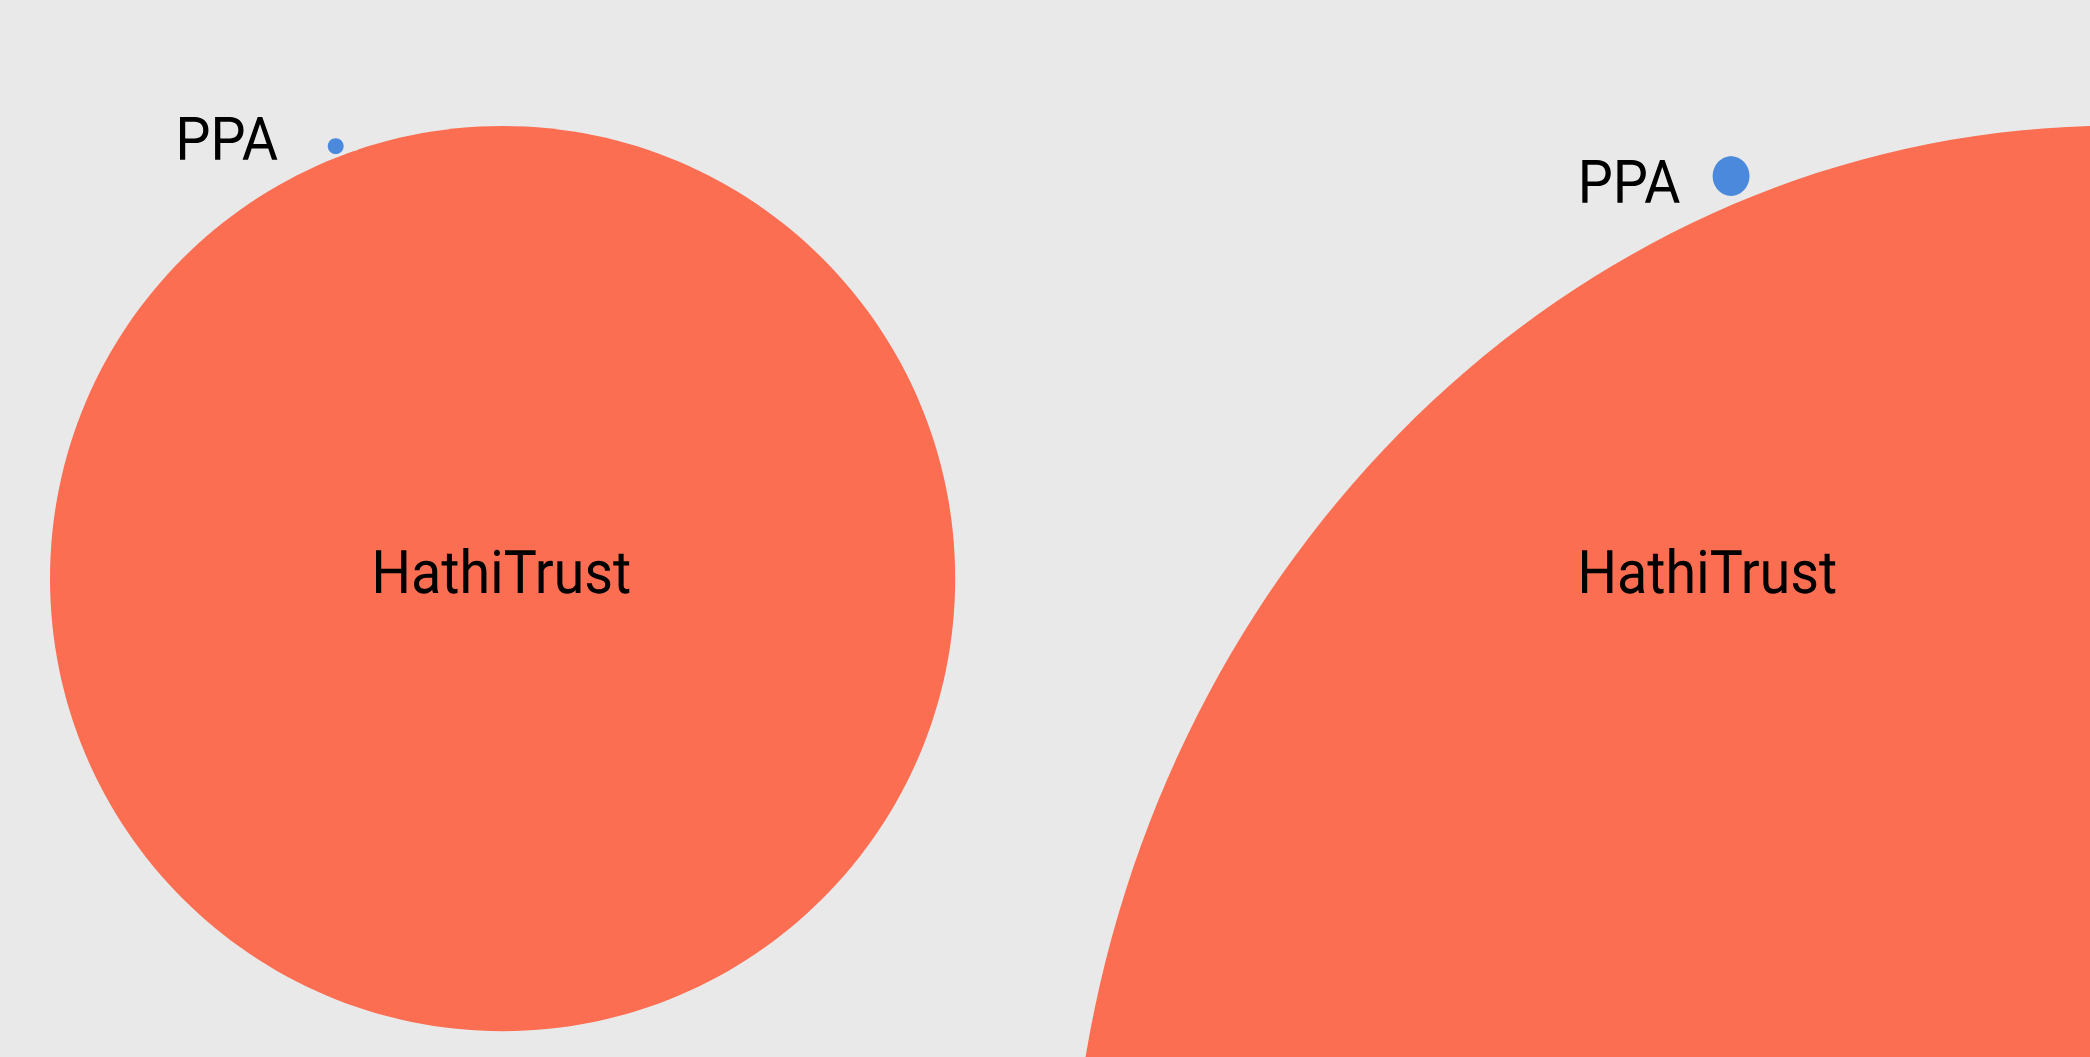
\includegraphics[width=0.75\linewidth]{figures/bubble-chart.png}
    \caption{This bubble chart, originally published in Rebecca Sutton Koeser’s essay “Visualizing the Collections,”\cite{koeser_visualizing_2020} shows the relative scale of HathiTrust and PPA as of 2020. At the time of writing, the PPA contains 5,480 HathiTrust works, or 0.025\% of HathiTrust. }
    \label{fig:bubble-chart}
\end{figure}
This vast difference in scale is actually a reason for the PPA’s creation; such a highly specialized discourse would easily get lost when searching the full scale of HathiTrust’s collection. Other, more standard collaborations with HathiTrust than ours share this same motivation. Many HathiTrust-based projects focused on various methods for, first, finding certain kinds of material within HathiTrust’s massive digital library, and then testing various text and data mining methods on that collection using the tools and services provided by HathiTrust Research Center (HTRC)\cite{noauthor_hathitrust_nodate}. Prominent examples of this two-step process include Gioia Stevens’s \textbf{Early American Cookbooks} project (now a permanent collection within HathiTrust) \cite{stevens_new_2017} and Laure Thompson and David Mimno’s \textbf{20th Century English-Language Speculative Fiction }(a recommended workset within HTRC) \cite{thompson_building_nodate} \cite{noauthor_recommended_nodate}. Recent work from Ryan Dubnicek and various collaborators has focused on using machine learning methods to discover particular genres within HathiTrust Digital Library \cite{parulian_uncovering_2022} \cite{dubnicek_ryan_piloting_2023} and building out the customizable capacities of HTRC’s Extracted Features dataset through the development of an open API \cite{john_a_walsh_library_nodate}. While this work has been important, the algorithms, datasets, and advanced computing environments are all contained within HTRC’s “walled garden,” a closed platform with controlled access and limited interactions. Part of what makes the case of the PPA so unusual is that it brings HathiTrust’s data out of the “walled garden” and puts it in conversation with works that are not found in HathiTrust: eighteenth-century tracts owned by Gale/Cengage, and early modern works from EEBO-TCP. We believe that working across walled gardens is the future of computational scholarship, as evidenced by the sunsetting of JSTOR’s TDM platform Constellate on July 1, 2025 \cite{noauthor_constellate_2019} and HathiTrust’s announcement in October 2024 that it was shutting down the HTRC because “many of our members have rarely utilized HTRC’s services,” leaving the future of TDM on HathiTrust works uncertain \cite{noauthor_plans_nodate}.

Cutting across walled gardens to incorporate works from Gale/Cengage’s ECCO into the PPA introduced different kinds of instability. Indeed, the ECCO data provides an interesting counterpoint to the instability of HathiTrust: the data itself is unchanged, and the OCR text for these materials have not been updated since 2008, even though there have been substantial improvements in OCR technology since the collection was originally digitized, in spite of the known poor quality of the text \cite{hill_quantifying_2019}. In this case, we encountered instability in the technical and human infrastructure. In the time since we first added the integration in 2021, Gale/Cengage made changes to its API that broke our image thumbnails, as well as the PPA links to ECCO for non-Princeton users. These changes required work on our part to adapt our systems and fix the issues. As with HathiTrust, we have also encountered personnel turnover, where our key contacts and collaborators have left without notice. Although our agreements with these institutions are formalized in MOUs, or Memoranda of Understanding, they generally view our project as an exception or experiment for an unusual use case, so there is no plan for continuity when our contacts leave, as Koeser, Naydan, and Martin have previously discussed \cite{naydan_beyond_2024}.

It is difficult to identify other digital projects with unusual uses of data or technical infrastructure from an outside perspective; this requires insider knowledge of the process of working with vendors to build projects, which is less often narrated than research methods, analytical results, or final outputs. Meredith Martin’s new monograph, \textit{Poetry’s Data}, is a notable exception to this trend and argues for the value of narrating the process of navigating our digital research infrastructures \cite{martin_poetrys_2025}. The Princeton Geniza Project and the Shakespeare \& Company Project are two additional examples of unexpected uses, since they both use IIIF in unintended ways \cite{noauthor_princeton_nodate, noauthor_shakespeare_2020}. 

\subsubsection{The problem of excerpts}

The most unusual aspect of PPA’s use of HathiTrust is arguably its support for book excerpts and journal articles. HathiTrust scans and indexes full works and full volumes of journals; it does not provide any consistent, reliable, or systematic semantic structure to identify the chapters or articles contained within them. After our initial launch in 2019, however, it quickly became clear that excerpt-level indexing would surface discoveries that would otherwise remain buried beneath unspecific metadata \cite{naydan_book_2024}. Between 2020 and 2021, the PPA project team worked to identify relevant journal articles and book chapters within larger works and curated the excerpt-level metadata manually. 

The integration of excerpts was how we realized the extent of the unstable data issue in the first place, as the team encountered mismatches between the thumbnail image and full-text snippets of excerpts while browsing the archive after excerpt support was implemented. Our previously correct page ranges were now wrong. How was this possible? As we discovered, the digital page ranges of content could shift due to the way we were dynamically pulling content from multiple HathiTrust systems whenever HathiTrust rescanned works in ways that introduced changes to the digital page numeration.

We suspect that HathiTrust’s regular rescanning of material is not widely known or even fully understood among researchers. The only public indication is the following disclaimer that HathiTrust includes on one of its “About” pages (emphasis added): "\textit{The HathiTrust collection is not static.} Works get added to the collection every day, and \textit{sometimes a digital item may be updated with a new version}. Bibliographic records can be updated when contributors send us corrections. Copyright and access statuses may change as items undergo copyright review or we receive permissions agreements from copyright holders" \cite{noauthor_how_nodate}.

HathiTrust’s “Full view” page for individual items also provides clues to changes. A  “Version” label with a date indicates when an item was last updated. However, this date could indicate a substantive change, like a full or more complete rescanning; a less obvious change, such as the addition of deep page-level metadata; or a trivial change, such as metadata corrections. There is no way to easily identify the type of change.

The project team began to brainstorm ways to automate fixing range changes for excerpts whenever HathiTrust made updates to works in the PPA. At first glance, it seems like a task that should be computationally tractable, and when we presented this unsolved problem to a junior computer science independent work seminar taught by Brian Kernighan, Kernighan thought so, too. His investigations \ref{fig:code-comparison} usefully illustrate the problem we faced: 

\begin{figure}
    \centering
    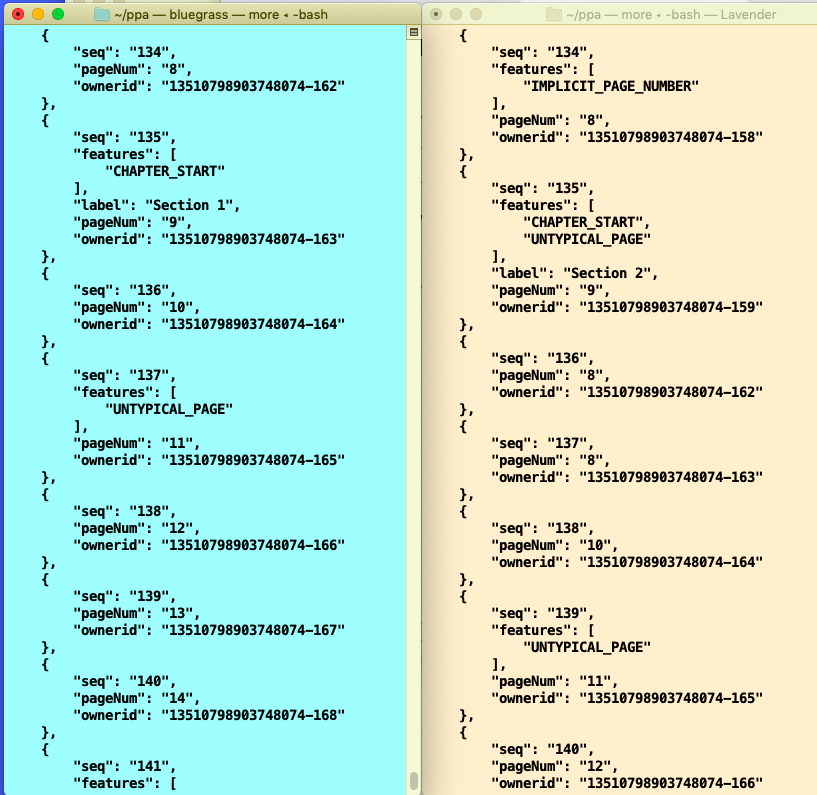
\includegraphics[width=0.5\linewidth]{figures/y.png}
    \caption{Side-by-side screenshots showing page-level metadata for “The Scansion of Middle English Alliterative Verse” by William E. Leonard \cite{noauthor_scansion_nodate}, generated from the page’s HTML and javascript, on two different dates: March 18, 2024 (left) and March 26, 2024 (right). Some of the changes involve recharacterizing page-level semantic metadata (e.g. flagging “UNTYPICAL\_PAGE” or section starts, though it is worth noting that these changes are not always more accurate). Note also the change in purported page numbers (“pageNum”) beginning with sequence (“seq”) 134. The OwnerID number, used in the permanent link to page scans, also changes relative to the accompanying sequence and page numbers.}
    \label{fig:code-comparison}
\end{figure}
Digging deeper, Kernighan discovered cases with particularly thorny issues with the page number metadata. For instance, the following page from O. F. Emerson’s “The Development of Blank Verse: A Study of Surrey” in the journal \textit{Modern Language Notes }displays \textit{three} different page numbers \cite{emerson_o_f_development_1889}:

\begin{figure}
    \centering
    \includegraphics[width=1\linewidth]{figures/Screenshot 2025-07-10 at 3.19.38 PM.png}
    \caption{Each column of \textit{MLN }gets its own page number (left, 467; right, 468), and each page gets a third, found at the bottom center (234). HathiTrust’s black navigation controls show that it interprets the upper left page number as the original/physical page number (p. 467) — hardly an intuitive choice. This means that scrolling through HathiTrust’s reader, the original page numbers increase by two instead of one. The digital page number/sequence number (\#296) is based on scanning and subject to change with rescanning.}
    \label{fig:MLN}
\end{figure}
It became apparent that automating page range fixes would not be trivial due to cases like these. Although there are certainly approaches that could help, our proposed solution involved flagging recently changed volumes for manual review. However, the ongoing human curation needed, in addition to the technical complexity, led us to decide that implementation was out of scope for that project.

\section{Quantifying HathiTrust’s rate of change}

\subsection{Changes in PPA excerpts}

A spreadsheet from November 2023 to correct the page ranges for PPA excerpts from HathiTrust provides a window into the degree of instability and changes we have encountered over a period of about two years. After we discovered that we were pulling erroneous content for some excerpts, we tasked a student researcher with manually checking and correcting the digital page range for excerpts that had shifted. Of 517 total excerpts, 121 excerpts (23.4\%) had changed. For 10 of those excerpts, the number of pages included changed; in these cases, the most common change was 2 pages.\footnote{There were two outliers with differences in length of 25 and 16 pages; preliminary investigations suggest that these were due to data errors in the original excerpts. For instance, one excerpt was originally only pulling a single page when the article was actually several pages long; someone neglected to input the end range. However, it is difficult to confirm with certainty after the fact.} While unusual, this might occur if, for instance, HathiTrust erroneously scanned the same page twice within an excerpt sequence, and then updated the scan to rectify the error. If we look at the difference in start pages between these updates, we find an average shift of 6.4 pages; 9 volumes shifted by more than 10 pages, 5 by more than 10, and one outlier, Thomas Stewart Omond’s “Swinburne as a Metrician” in volume 76 (1909) of \textit{The Academy and literature}\cite{omond_thomas_stewart_swinburne_1909}, shifted by 240 pages! This could happen if HathiTrust was initially missing an issue or two from a full run of that year’s journal, and added it later in a rescanning. Most troubling, when we analyze the overlap between pages in range before and after these updates, \textit{there are 36 excerpts with no pages in common between the initial and updated page range}; that is, without updating the page range, we would be including \textit{none} of the intended contents.

\subsection{Changes in all of HathiTrust}

Observing this volatility at the small scale of PPA excerpts led us to wonder about the rate of change for  PPA content more generally and in HathiTrust at scale. Fortunately for us, HathiTrust is incredibly transparent and publishes monthly and daily files with data about updated records, including a list of the reasons a volume might be included, whether newly deposited, a new copy of an existing item, changes to rights and access permission, or an update to the bibliographic metadata \cite{noauthor_hathifiles_nodate} .  Figure \ref{fig:hathi-daily-updates} charts the number of updated volumes across all of HathiTrust from May 1 to July 10, 2025.
\begin{figure}[t!]
    \centering
    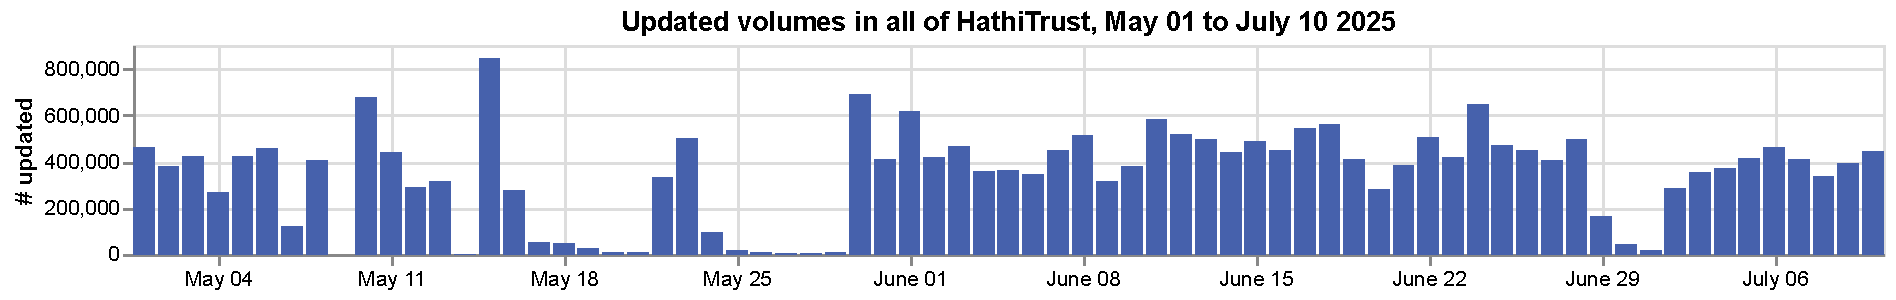
\includegraphics[width=1\linewidth]{figures/hathitrust_changes_countonly.pdf}
    \caption{Number of volumes updated daily in all of HathiTrust from May 1 to July 10, 2025.}
    \label{fig:hathi-daily-updates}
\end{figure}
The number of updates varies on any given day from nearly negligible to more than 800,000 volumes. The day with the most updates during this time period was May 15, 2025 with 846,329 volumes updated (4.5\% of all HathiTrust).  However, at HathiTrust’s scale of 18+ million volumes, the changes constitute less than 1\% of the total collection. 

\subsection{Changes in all of the PPA}

What about all the HathiTrust volumes within the Princeton Prosody Archive? How frequently are they changing? One way to answer this question is to filter the data on HathiTrust updates to volumes included in PPA; when we do, we find that PPA updates track somewhat with the larger updates (refer to Figure \ref{fig:ppa-daily-updates} and compare with Figure \ref{fig:hathi-daily-updates}). Although these changes are on a much smaller scale, there are still multiple days when more than a hundred volumes changed within this time period.

\begin{figure}[t!]
    \centering
    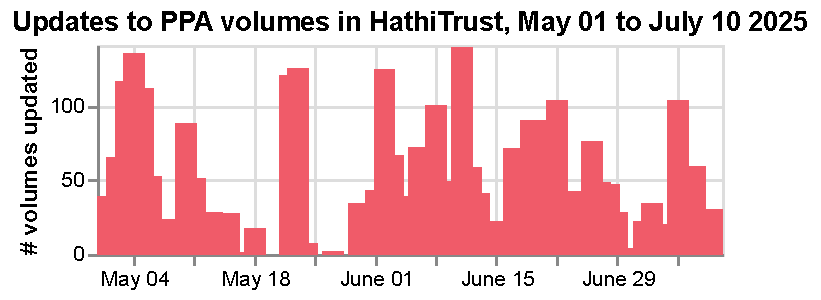
\includegraphics[width=1\linewidth]{figures/ppa_hathitrust_changes_countonly.pdf}
    \caption{Number of PPA volumes updated daily in all of HathiTrust from May 1 to July 10, 2025.}
    \label{fig:ppa-daily-updates}
\end{figure}

To answer this question, we compared two different snapshots of the PPA full-text corpus: one from 2025-02-03 (when did we last run rsync for this one?), and the other from 2025-02-19, a difference of roughly two weeks. Within this time frame, close to half of our pages (44.2\%) changed after joining on page ID (work ID + digital page sequence number). Another way of looking at the rate of change within the PPA corpus involves joining the matching text within a volume to see whether page ID has changed. Via this method, 855,930 pages have exactly matching text in both versions. For just 14,423 of those pages (1.7\%), the page id has changed. This is the set of pages where the digital sequence has changed without OCR changes. For the remaining \~half a million (is this right?) pages in the set, those mismatches can likely be attributed to OCR changes.

\begin{figure}[t!]
    \centering
    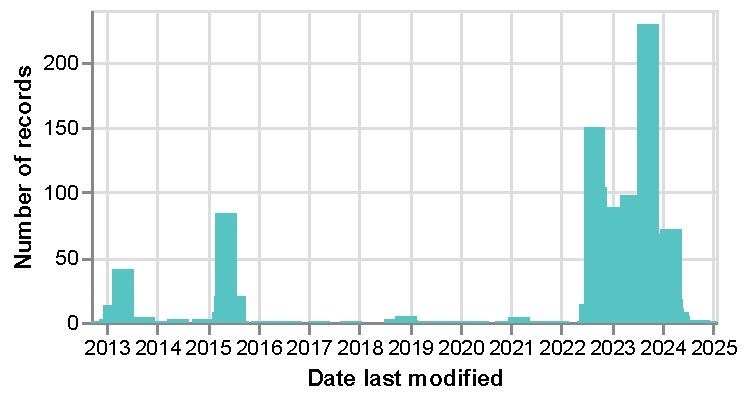
\includegraphics[width=1\linewidth]{figures/ppa_hathitrust_lastmodified.pdf}
    \caption{Last modification date of PPA content files.}
    \label{fig:ppa-last-modified}
\end{figure}

\subsection{Implications}

When PPA research efforts shifted from data aggregation, curation, and presentation to computational analysis based on the PPA text corpus, we had new opportunities to engage with and build on prior research; however, this made the repercussions of the instability of our source data much more obvious. PPA researchers identified an initial corpus-wide research project to detect and identify lines of poetry quoted across the million+ pages. The PPA consists of writing \textit{about }poems, and these texts often include lines of poetry to underscore or illustrate a particular prosodic term or metrical feature. Systematically identifying these quoted poems was a first step towards answering research questions about English prosody; for instance, a dataset of poem excerpts cited in the PPA could illuminate when and how particular poets or poems became the exemplars for particular poetic forms or figures of speech, or how quickly after publication a poet’s work is canonical enough to be discussed as an example of prosody, or to trace the network of examples being picked up and reused from other prosodists.

As we considered possible approaches to the problem of poetry detection at scale, one collaborator suggested making use of a dataset of page-level genre predictions for HathiTrust volumes created by Ted Underwood \cite{underwood_page-level_2014}. This dataset includes page-level predictions because, as the researchers note, volumes are rarely a single genre and often include collections of disparate materials. While the genre prediction task is not strictly the same as poetry detection, there is enough overlap that data on pages predicted as poetry could be used as a starting point or confirmation of results from other methods. However, the degree of change possible in HathiTrust materials means that this page-level data is basically unusable; there may be volumes included where the pages have not changed, but determining which ones those are would be difficult. As a demonstration of this problem, we offer one example. The essay “On Stile and Versification” by William Belsham\cite{belsham_stile_1799} is one of the excerpts included in PPA with known poetry excerpts; many of the pages include short poetry quotations, and there are two pages in sequence that are all or almost all poetry. Nearly all of the pages in this volume are classified as nonfiction prose in the page-level genre dataset, except for two pages in sequence that are labeled as poetry near the page range of this excerpt. However, the page indexes don’t match any of the expected pages in our data. In Underwood’s page-level genre metadata, the poetry pages are numbered 510 and 511. In our current volume, the digital pages are 515 and 516; the original printed pagination is 507 and 508).

\begin{figure}[hbt!]
  \centering
  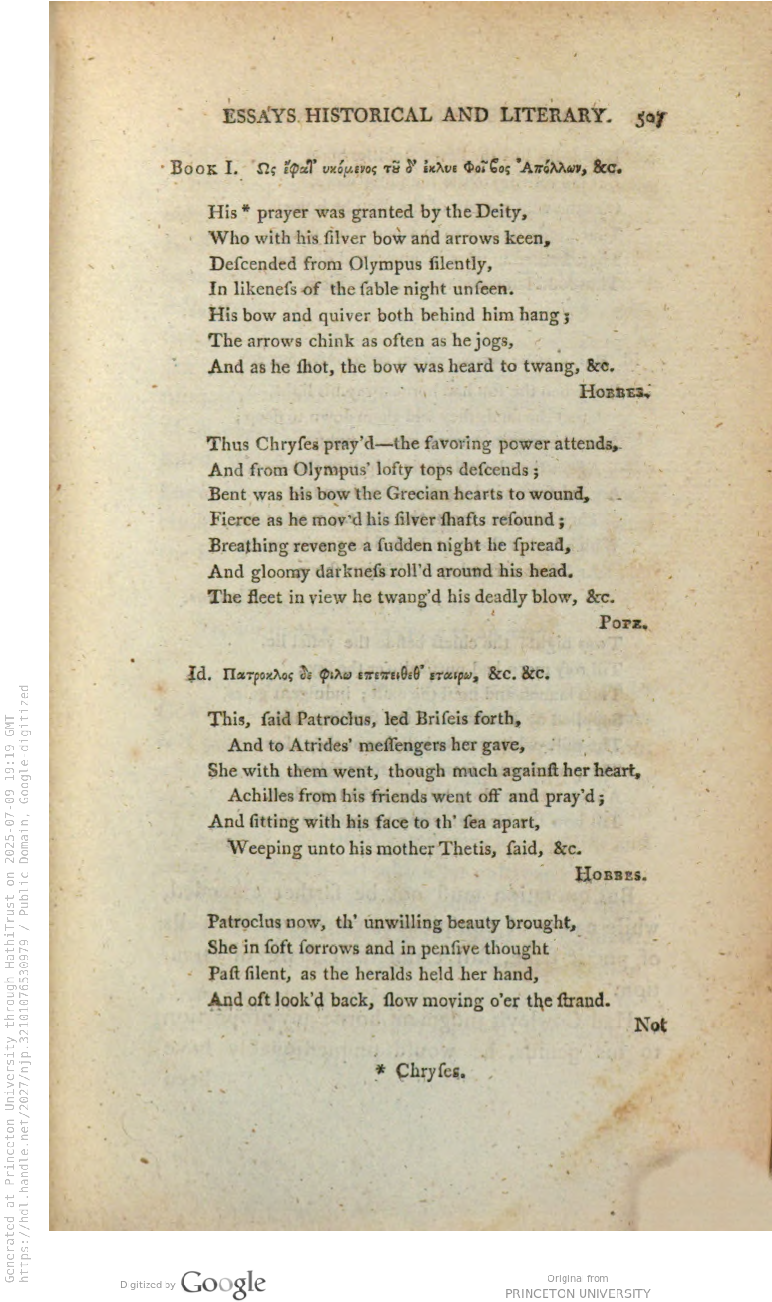
\includegraphics[width=0.35\linewidth]{figures/hathi-pages/njp-32101076530979-515-1752088772.pdf}
  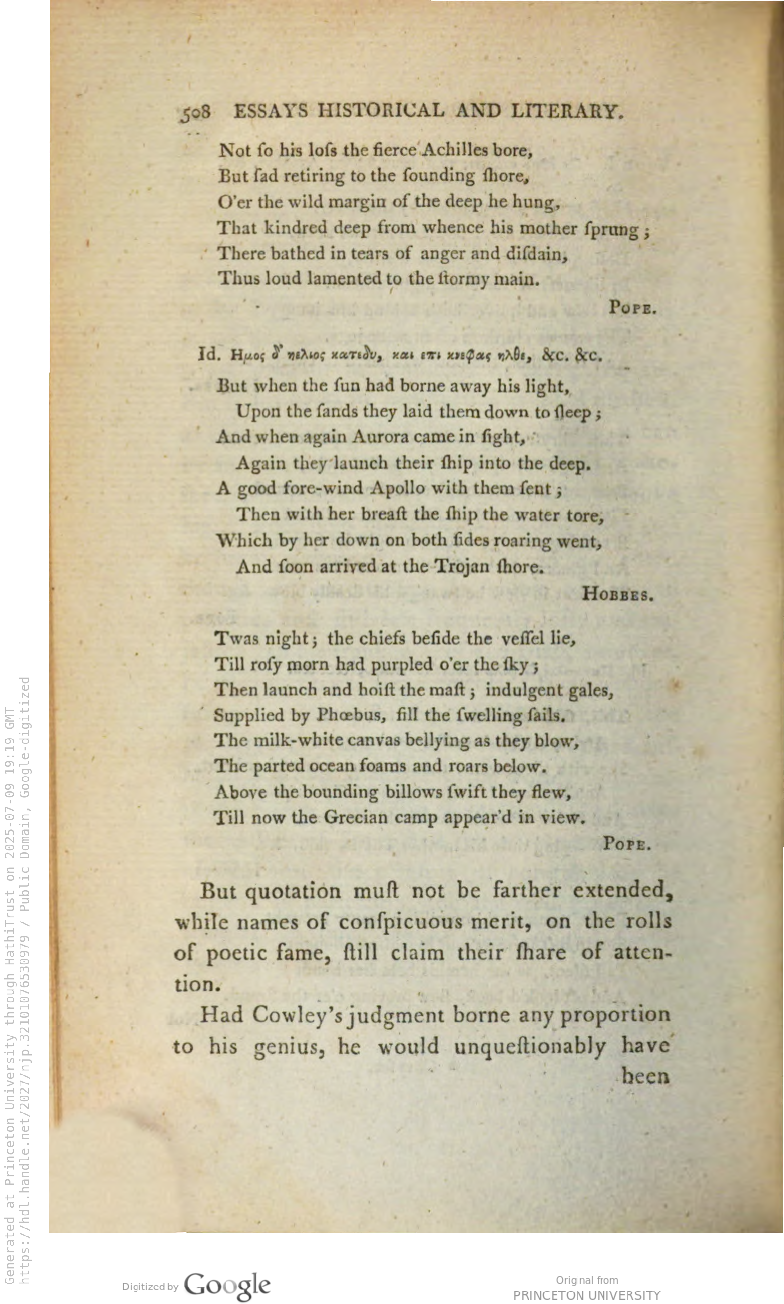
\includegraphics[width=0.35\linewidth]{figures/hathi-pages/njp-32101076530979-516-1752088741.pdf}
  \caption{Two pages of all or almost all poetry with page-level genre labels of poetry.}
  \label{fig:poetry_pages}
\end{figure}

\begin{figure}[hbt!]
  \centering
  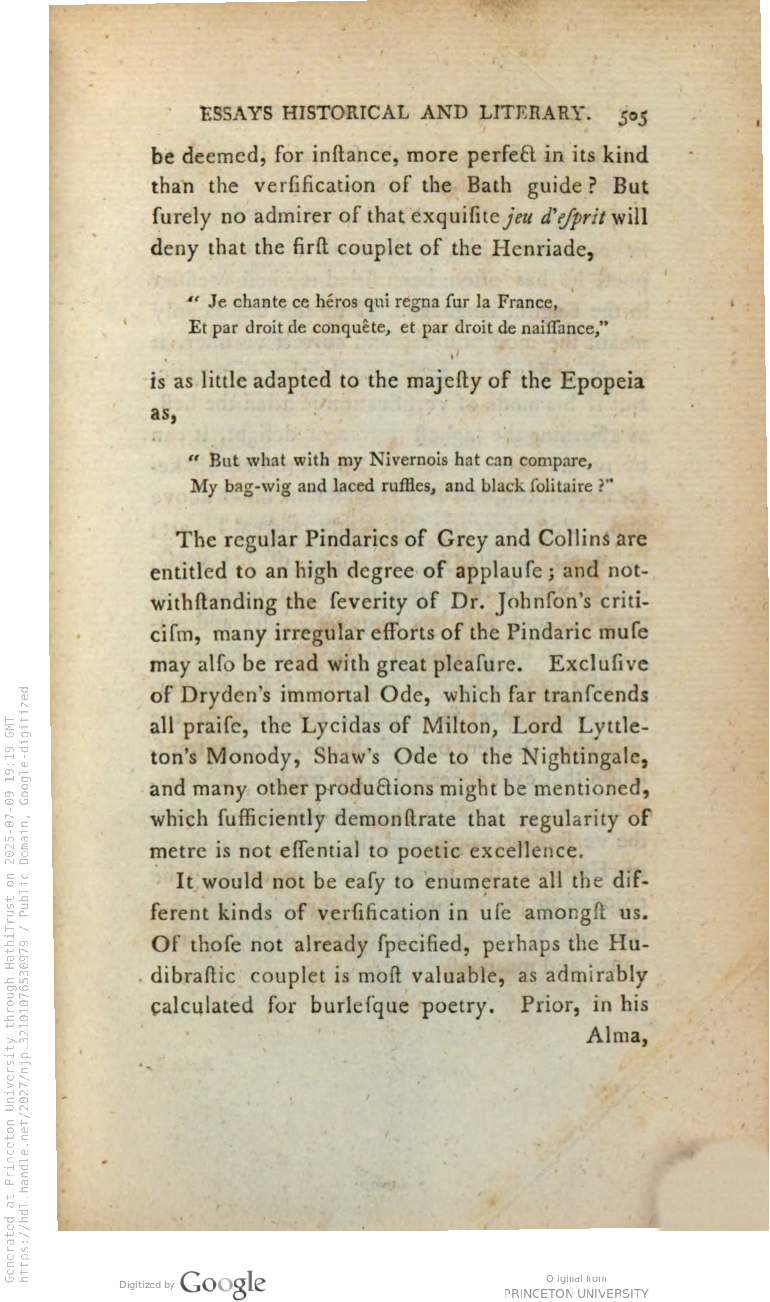
\includegraphics[width=0.35\linewidth]{figures/hathi-pages/njp-32101076530979-513-1752088792.pdf}
  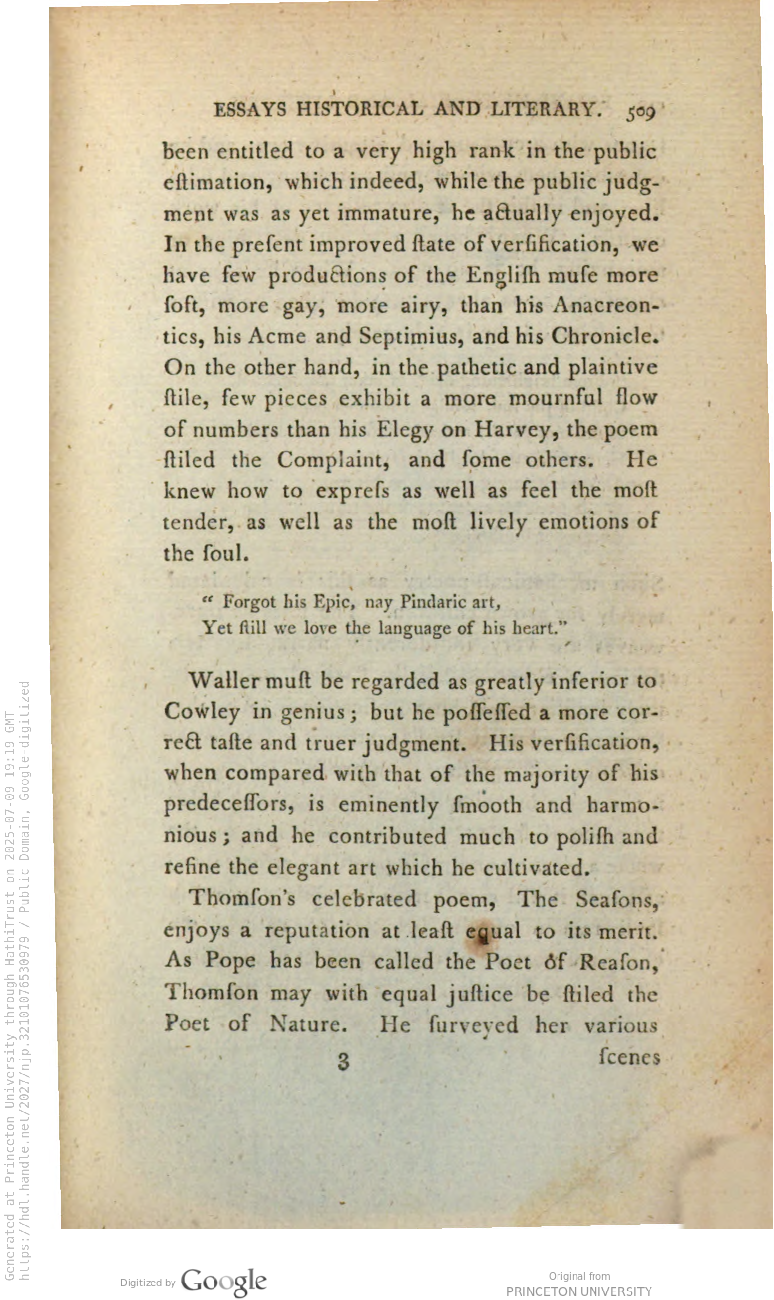
\includegraphics[width=0.35\linewidth]{figures/hathi-pages/njp-32101076530979-517-1752088752.pdf}
  \caption{Two pages with short poetry excerpts not labeled at the page level as poetry.} Images courtesy of HathiTrust. 
  \label{fig:poetry_exc_pages}
\end{figure}
The conclusions we draw from this example are that page-level genre predictions could be used to identify pages within PPA that are substantially poetry, which would be useful for some research questions and data curation tasks, and could provide partial information for the poetry detection task, but the updates to HathiTrust content since that dataset was published make it unusable for work on current copies of HathiTrust data.

Like Underwood, the PPA project team is using digital sequence to refer to pages in our found-poems dataset. What do we do with the fact that this dataset, like Underwood’s, refers to a snapshot of HathiTrust and the PPA at a moment in time? For researchers working with HathiTrust data, there is no stable page identifier across time. A stable page ID for HathiTrust is not feasible due to the scale of labor involved in creating and maintaining HathiTrust, since there are so many individual libraries with their own workflows feeding into the aggregator. While this lack of stable referents is therefore understandable, it nevertheless poses a problem for computational research and reproducibility that the field has yet to solve. 

\section{Conclusions}

There are many different modes of computational research on large-scale corpora like HathiTrust. The difficulty of dealing with the frequent changes made by HathiTrust and Gale/Cengage was a big part of our decision to shift from maintaining a dynamic database to extracting the data and analyzing the full-text corpus instead. In doing so, we are engaging in a familiar mode of computational scholarship: working with a frozen snapshot of a corpus at a particular moment in time to test a method or transform it into a different kind of data. This mode has the benefit of being versioned; you can point to the version of the dataset you used for your research, and sometimes even share it depending on permissions. However, this mode of scholarship prevents us from building on one another’s work. It is its own kind of walled garden, failing to feed back into or truly enhance collections like HathiTrust, Gallica, or TROVE. As long as we are doing computational research on bespoke datasets, our work doesn’t make it out of the garden, either for application in the GLAM sector or to advance domain research. 

When it is working well, GLAM data and research constitute a virtuous cycle: the data feeds the research, and then the research improves the data for everyone, as well as making research domain arguments. However, this loop is rarely so well-oiled. More frequently, the goals of the institution and the researcher are mismatched. For instance, the PPA’s unusual use of HathiTrust to dynamically present excerpts would benefit from a semantic division of texts into meaningful parts. For HathiTrust, that level of detail is not needed to achieve its goal of providing “reading access,” and it is not feasible at the massive scale at which they are working. Considering their scale of operation, HathiTrust and other aggregators have done a remarkably good job of being transparent about high-level changes to their collections: sending emails to indicate deletions and tracking updates through a version label. They have also done a remarkable job supporting the rather niche work of computational humanists, and the closure of Constellate and HTRC suggests they did this with little return on the investment. In the absence of aligned goals, perhaps the best we can do as researchers is to be equally transparent: to inform other researchers about the instabilities and limitations we discover in the collections we are working with, and to publish and share versioned data to the fullest extent possible. 


\section*{Acknowledgements}

This unnumbered section should be blank when submitting your paper. After review, you may include lists of people and organizations who supported the work.

% Print the biblography at the end. Keep this line after the main text of your paper, and before an appendix. 
\printbibliography

% You can include an appendix using the following command
\appendix

\section{HathiTrust Statement for Dataset Distribution} \label{appdx:first}

By my signature, I acknowledge and confirm the following:

\begin{enumerate}
    \item  I am receiving texts from the University of Michigan that are made available under an agreement between my sponsoring institution - [indicate sponsoring institution, e.g., Dartmouth College] - and Google.
    \item  I have read this agreement and agree to abide by its terms and to use the texts in accordance with the statement of my research, as submitted to the University of Michigan.
    \item  I agree to notify the University of Michigan of any changes that are made in the scope or nature of my research.
    \item  I understand that volumes I receive from the University of Michigan may be determined at a later date to be in copyright. I agree to delete these volumes and any copies that have been made upon notification from the University of Michigan. I agree to notify the University of Michigan at feedback@issues.hathitrust.org to confirm deletion of any such volumes.
\end{enumerate}

\rule{\textwidth}{0.5pt}

Name \hspace{0.3\textwidth} Signature \hspace{0.3\textwidth} Date

\rule{\textwidth}{0.5pt}

Title

\rule{\textwidth}{0.5pt}

Email \hspace{0.3\textwidth}  Phone


\section{Example HathiTrust deletion email for public domain dataset} \label{appdx:second}

\begin{verbatim}
Subject: Delete notifications for ht_text_pd dataset
From: HathiTrust <support@hathitrust.org>

Dear HathiTrust dataset recipient,

This email is to notify you that volumes in the HathiTrust
"ht_text_pd" dataset, of which you have downloaded all
or a subset of files, no longer meet the criteria for
inclusion in the dataset, and you no longer are allowed to
use them in your research.

Please review the data you have synced from HathiTrust to
check whether you have the volumes listed below. If so,
delete all copies you retain of these volumes in
accordance with our terms of use. Alternatively, you may
delete your copy of the dataset and re-sync to the updated
dataset.

If you no longer possess HathiTrust datasets, or if you
have other questions regarding datasets, then please email
support@hathitrust.org.

Thank you,

HathiTrust

===BEGIN ID LIST===
[ids omitted]
...
...
...
===END ID LIST===

\end{verbatim}
\end{document}
